\chapter{Capitolo 4: Algoritmi basati sulla distanza}
In questo capitolo vengono illustrati i principali algoritmi utilizzati per la costruzione degli alberi evolutivi. L'obiettivo è quello di trovare una soluzione al cosiddetto \textit{problema degli alberi basati sulla distanza}, ma prima è necessario introdurre alcuni concetti, tra cui la matrice delle distanze.

\section{Matrice delle distanze}
Dati due punti, $x$ e $y$, la \textit{distanza} può essere vista come loro "lontananza" in uno spazio $k$-dimensionale. Nella fattispecie, è una funzione $d(x,y)$ che possiede le seguenti proprietà \cite{molaCagliari}:
\begin{enumerate}
	\item \textit{non negatività}:
	\[d(x,y)\geq 0\hspace{2em} \forall \: x,y\in R^k\]
	\item \textit{identità}:
	\[d(x,y)=0 \; \leftrightarrow \; x=y\]
	\item \textit{simmetria}:
	\[d(x,y)=d(y,x)\hspace{2em} \forall \: x,y\in R^k\]
	\item \textit{disuguaglianza triangolare}:
	\[d(x,y)\leq d(x,z)+d(y,z)\hspace{2em} \forall \: x,y,z\in R^k\]
\end{enumerate}
Date $n$ unità, calcolando la distanza per ogni coppia di elementi\footnote{Ci sono vari modi per calcolare la distanza tra una coppia di elementi, ad esempio attraverso la distanza Euclidea, quella di Manhattan, di Minkowski e così via.} si ottiene una \textit{matrice delle distanze $n \times n$}, definita nel seguente modo \cite{ingrassiaStatistica}:
\[
D = \begin{pmatrix}
0 & d_{12} & d_{13} & \ldots & d_{1n} \\ 
d_{21} & 0 & d_{23} & \ldots & d_{2n} \\ 
d_{31} & d_{32} & 0 & \ldots & d_{3n} \\ 
\vdots & \vdots & \vdots & \ddots & \vdots \\ 
d_{n1} & d_{n2} & \ldots & \ldots & 0
\end{pmatrix}
\hspace{3em}dove\;d(x_i,x_j)=d_i,_j
\]
Poiché è costruita a partire dalle distanze, ne eredita le proprietà precedentemente elencate.
\newline
Ciascun valore $d_i,_j$ può assumere significati diversi in base al contesto, ad esempio, può indicare il numero di simboli diversi tra i geni $i$ e $j$ nell'allineamento di sequenze di DNA\footnote{'allineamento è il processo attraverso il quale si misura la similarità tra due o più sequenze.}, come mostrato nell'esempio sottostante:
\begin{figure}[h!]
	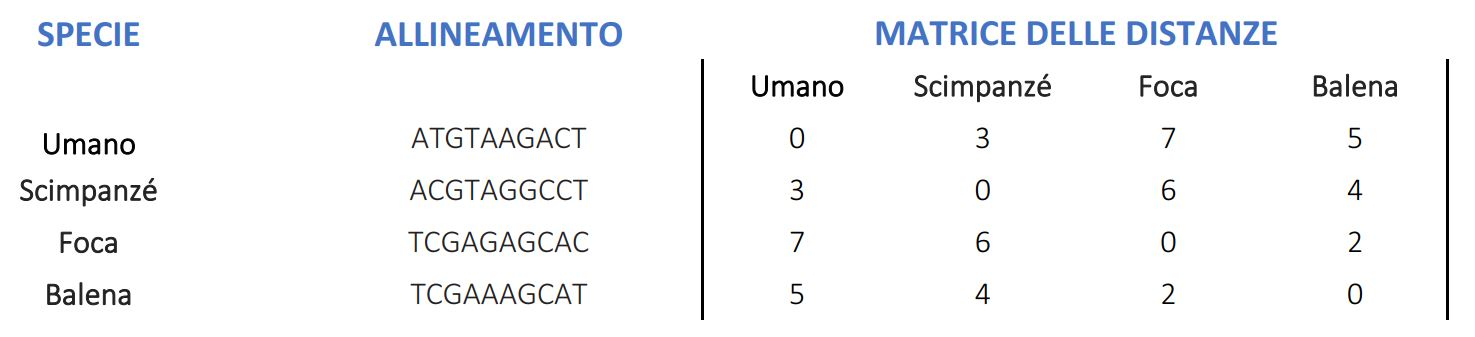
\includegraphics[width=\linewidth]{distance_matrix_example.jpg}
 	\caption{Esempio di matrice delle distanze.}
  	\label{fig:DistanceMatrix}
\end{figure}
\newline
Dalla figura 5 è possibile notare che la sequenza di DNA della foca risulta molto più simile a quella della balena, in quanto la distanza è $2$, piuttosto che con l'umano, la cui distanza invece è $7$.
\newpage

\section{Problema degli alberi basati sulla distanza}
Gli algoritmi basati sulla distanza utilizzano la matrice delle distanze per costruire gli alberi evolutivi, dove le foglie corrispondono alle entità biologiche presenti nella matrice, mentre i nodi interni rappresentano gli antenati non noti. Per poter conoscere quale è la distanza tra due foglie, e quindi conoscere quanto sono legate tra loro, è necessario associare un valore non negativo (peso) a ciascun arco, pertanto la lunghezza del cammino in tale albero è la somma dei suoi pesi. Si definisce, quindi, la \textit{distanza evolutiva} tra due entità biologiche corrispondenti alle foglie $i$ e $j$ di un albero $T$ come la lunghezza dell'unico cammino che li collega, ed è indicato come $d_i,_j(T)$ \cite{bioinfalganactivelearningapproachparttwo}. In altre parole è dato dalla somma dei pesi degli archi che ci sono tra $i$ e $j$.
\newline
Si dice che un albero $T$ si \textit{adatta} ad una matrice delle distanze $D$ se per ogni coppia di foglie $i$ e $j$ si ha che $d_i,_j=d_i,_j(T)$, ovvero l'elemento nella riga $i$ e colonna $j$ è uguale alla lunghezza del cammino che le collega (distanza evolutiva), in tal caso la matrice viene definita \textit{additiva}. Qualora invece non esista un albero che si adatti alla matrice, allora è \textit{non additiva}.
\newline
Si riporta di seguito un esempio che mostra un albero che si adatta alla matrice delle distanze mostrata nella sezione precedente.
\begin{figure}[h!]
	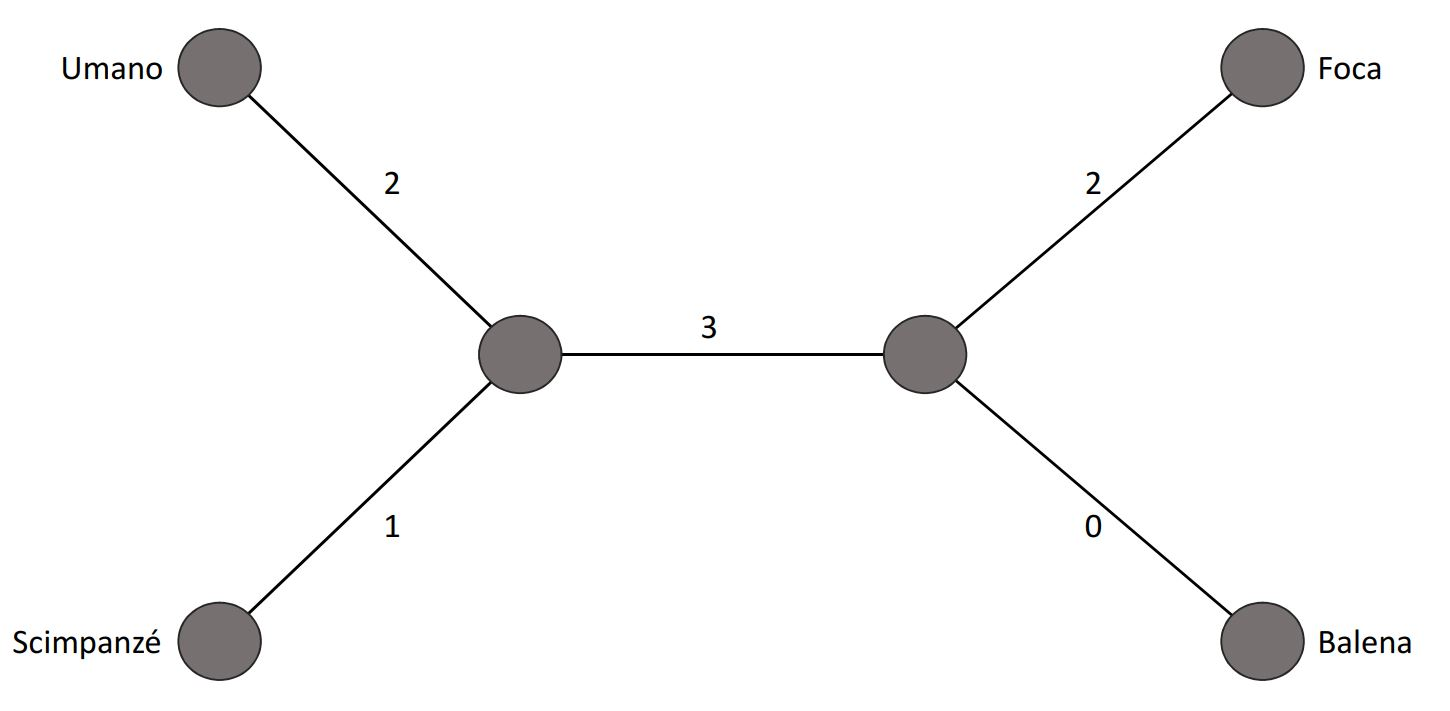
\includegraphics[width=\linewidth]{unrooted_tree_created_by_figure_5.jpg}
 	\caption{Albero evolutivo senza radice costruito a partire dalla matrice \textbf{adattiva} della figura 5.}
  	\label{fig:EvolutionaryTreeExample}
\end{figure}
\newline
Ci possono essere più alberi che si adattano ad una matrice, quindi come si può scegliere l'albero giusto? Si nota che quello in figura 6 ha tutti i vertici di grado diverso da due e viene definito \textit{albero semplice}. 
\newpage
Una loro caratteristica importante è che per ogni matrice delle distanze adattiva esiste un unico albero semplice che si adatta alla matrice stessa.
\newline
Adesso è possibile dare una definizione al problema accennato all'inizio del capitolo:
\begin{center}
\textbf{Problema degli alberi basati sulla distanza:}
\newline
\textit{Dato in \textbf{input} una matrice delle distanze adattiva si ottiene in \textbf{output} un albero evolutivo semplice.}
\end{center}

\section{Algoritmo per il problema degli alberi basati sulla distanza}
L'obiettivo è quello di costruire un albero semplice $T$ che si adatti alla matrice delle distanze $D$.
\newline
Si prenda in considerazione la matrice delle distanze mostrata nella figura 5:
\[
D = \bordermatrix{\text{specie}&u&s&f&b\cr
                u& 0 & 3 & 7 & 5\cr
                s& 3 & 0 & 6 & 4\cr
                f& 7 & 6 & 0 & 2\cr
                b& 5 & 4 & 2 & 0}
\]
Per brevità si definisce ,u=umano, s=scimpanzé, f=foca, b=balena.
\newline